%%%%%%%%%%%%%%%%%%%%%%%%%%%%%%%%%%%%%%%%%
% LaTeX Template
% http://www.LaTeXTemplates.com
%
% Original author:
% Linux and Unix Users Group at Virginia Tech Wiki 
% (https://vtluug.org/wiki/Example_LaTeX_chem_lab_report)
%
% License:
% CC BY-NC-SA 3.0 (http://creativecommons.org/licenses/by-nc-sa/3.0/)
%
%%%%%%%%%%%%%%%%%%%%%%%%%%%%%%%%%%%%%%%%%

%----------------------------------------------------------------------------------------
%	PACKAGES AND DOCUMENT CONFIGURATIONS
%----------------------------------------------------------------------------------------

\documentclass[12pt]{article}
\usepackage{geometry} % Pour passer au format A4
\geometry{hmargin=1cm, vmargin=1cm} % 

\usepackage{graphicx} % Required for including pictures
\usepackage{float} % 

%Français
\usepackage[T1]{fontenc} 
\usepackage[english,francais]{babel}
\usepackage[utf8]{inputenc}
\usepackage{eurosym}
\usepackage{lmodern}
\usepackage{url}
\usepackage{multicol}

%Maths
\usepackage{amsmath,amsfonts,amssymb,amsthm}
%\usepackage[linesnumbered, ruled, vlined]{algorithm2e}
%\SetAlFnt{\small\sffamily}

%Autres
\linespread{1} % Line spacing
\setlength\parindent{0pt} % Removes all indentation from paragraphs

\newcommand{\horrule}[1]{\rule{\linewidth}{#1}} % Create horizontal rule 
\renewcommand{\labelenumi}{\alph{enumi}.} % 
\pagestyle{empty}
%----------------------------------------------------------------------------------------
%	DOCUMENT INFORMATION
%----------------------------------------------------------------------------------------
\begin{document}

%\maketitle % Insert the title, author and date

\textbf{Nom(s), Prénom(s) :}

\begin{center}
\textit{La vie c'est comme une bicyclette, il faut avancer pour ne pas perdre l'équilibre.} - \textbf{Albert Einstein}
\end{center}

\begin{multicols}{3}

  \subsection*{Exercice 1}
  Les triangles suivants sont rectangles.\\
  \textbf{Écrire les égalités du théorème de Pythagore.}

  \begin{figure}[H]
    \centering
    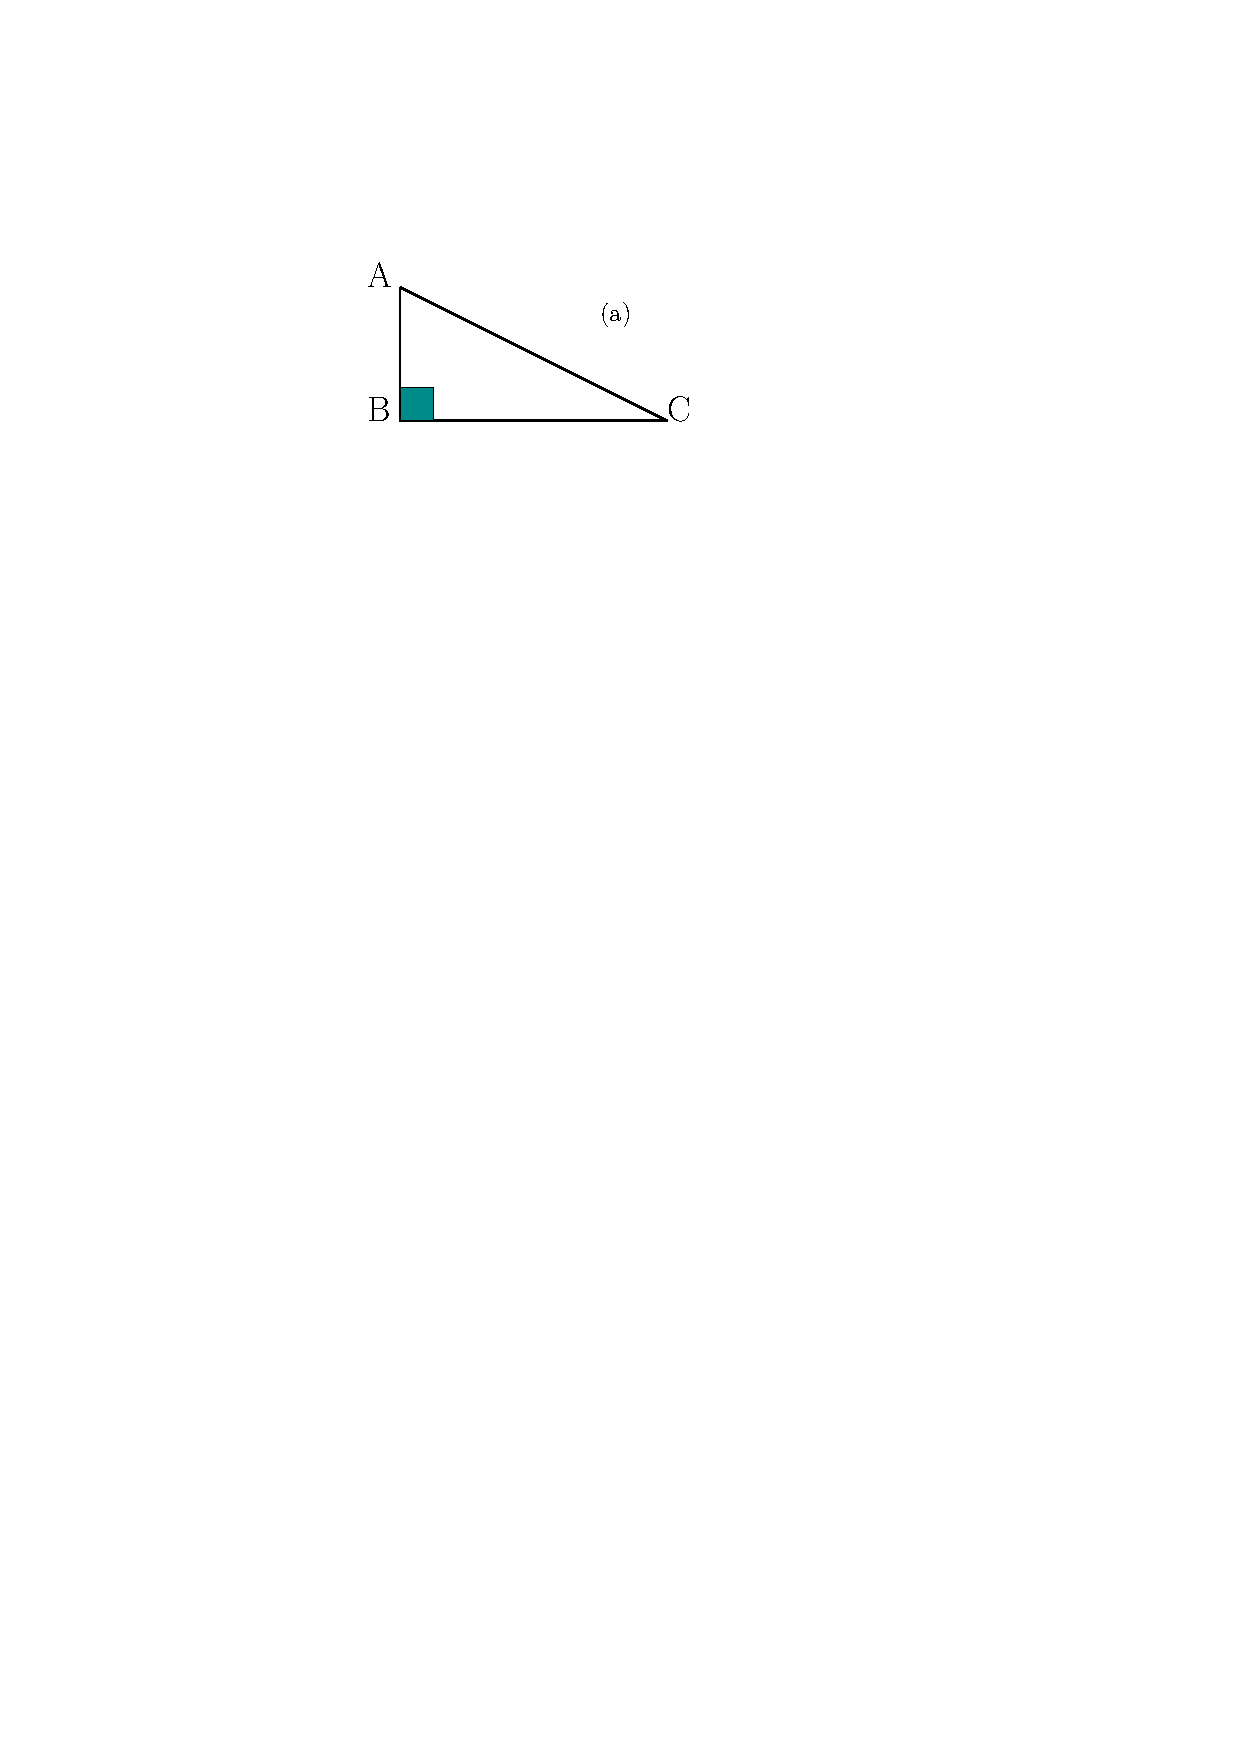
\includegraphics[width=0.7\linewidth]{sources/1/exo1-tri-1a.pdf}
  \end{figure}

  \begin{figure}[H]
    \centering
    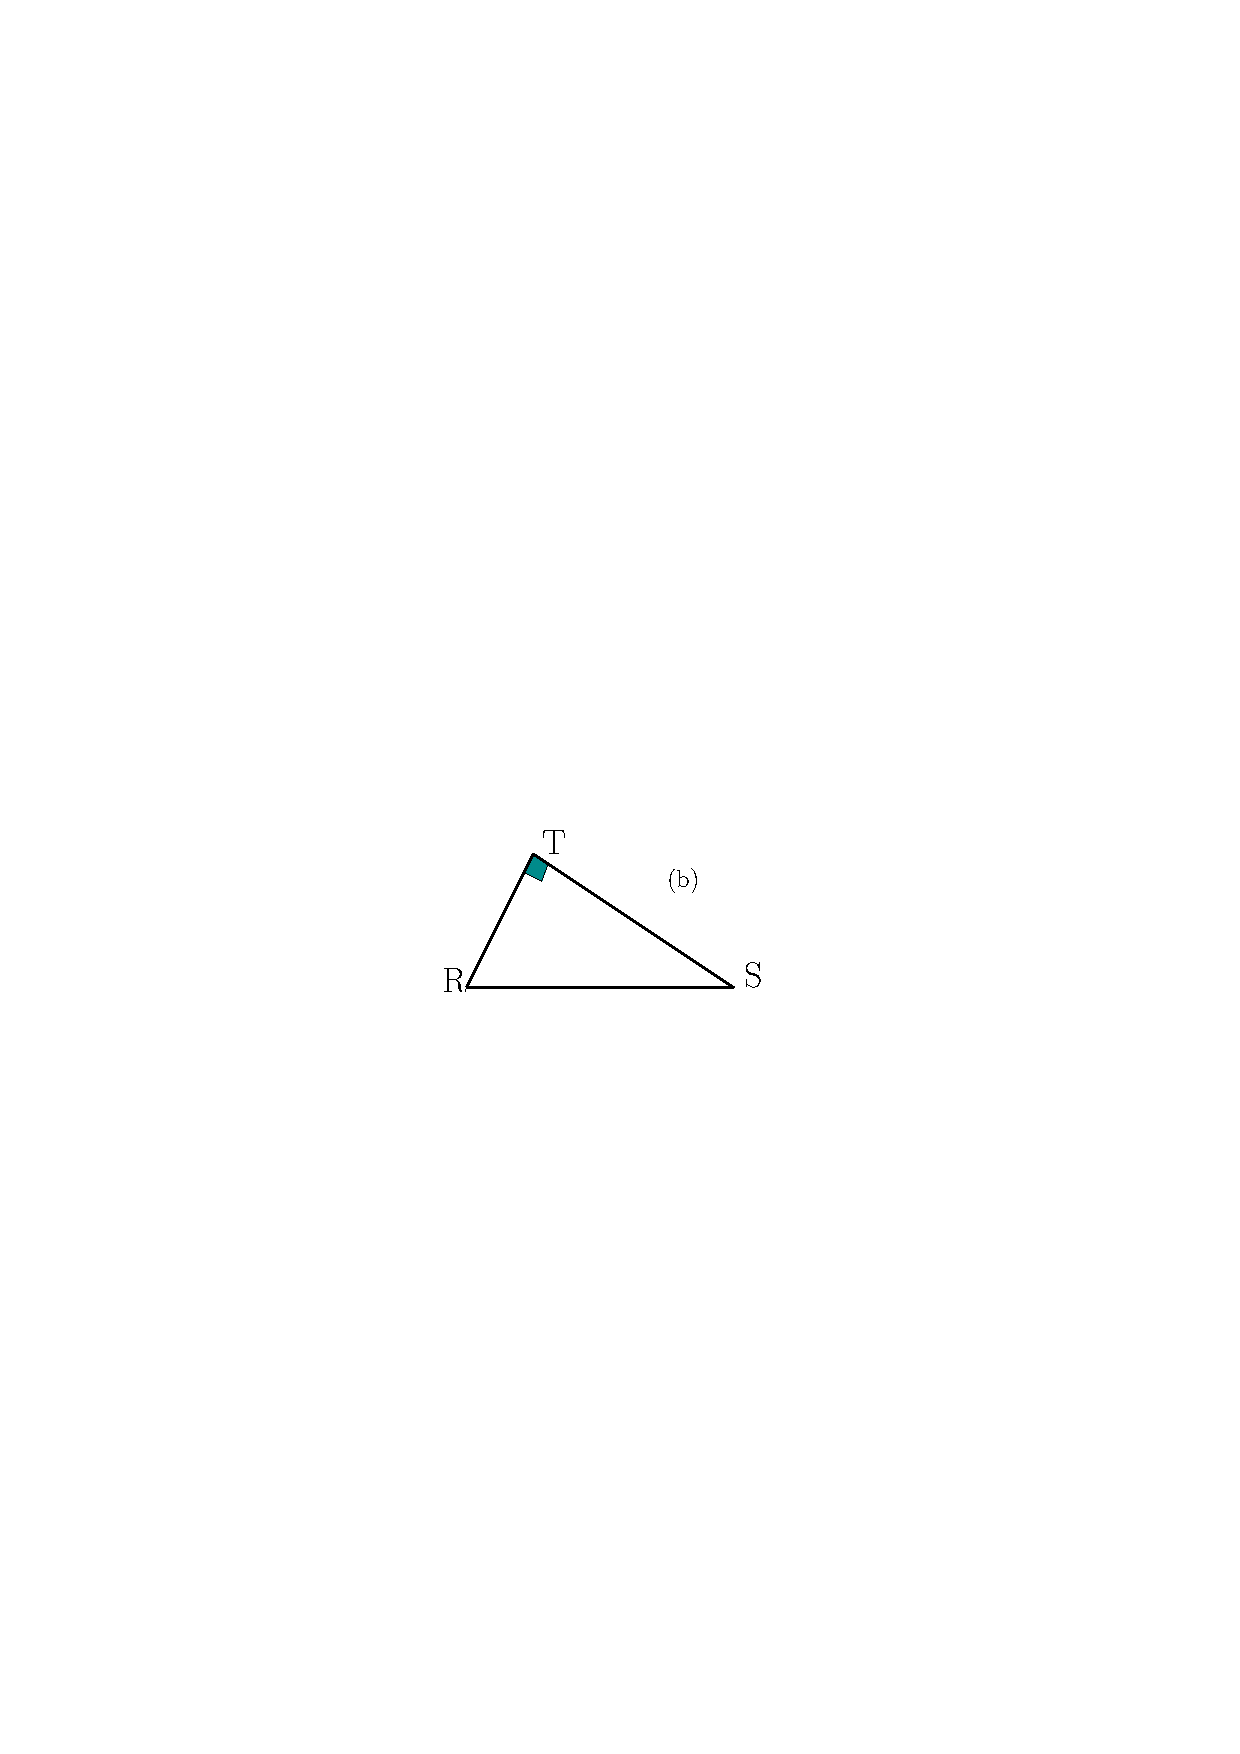
\includegraphics[width=0.7\linewidth]{sources/1/exo1-tri-2a.pdf}
  \end{figure}
  
\end{multicols}

\horrule{1px}

\begin{multicols}{3}

  \subsection*{Exercice 2}
  \textbf{Les triangles suivants sont-ils rectangles ?} \textit{Justifier.}
  
  \begin{figure}[H]
    \centering
    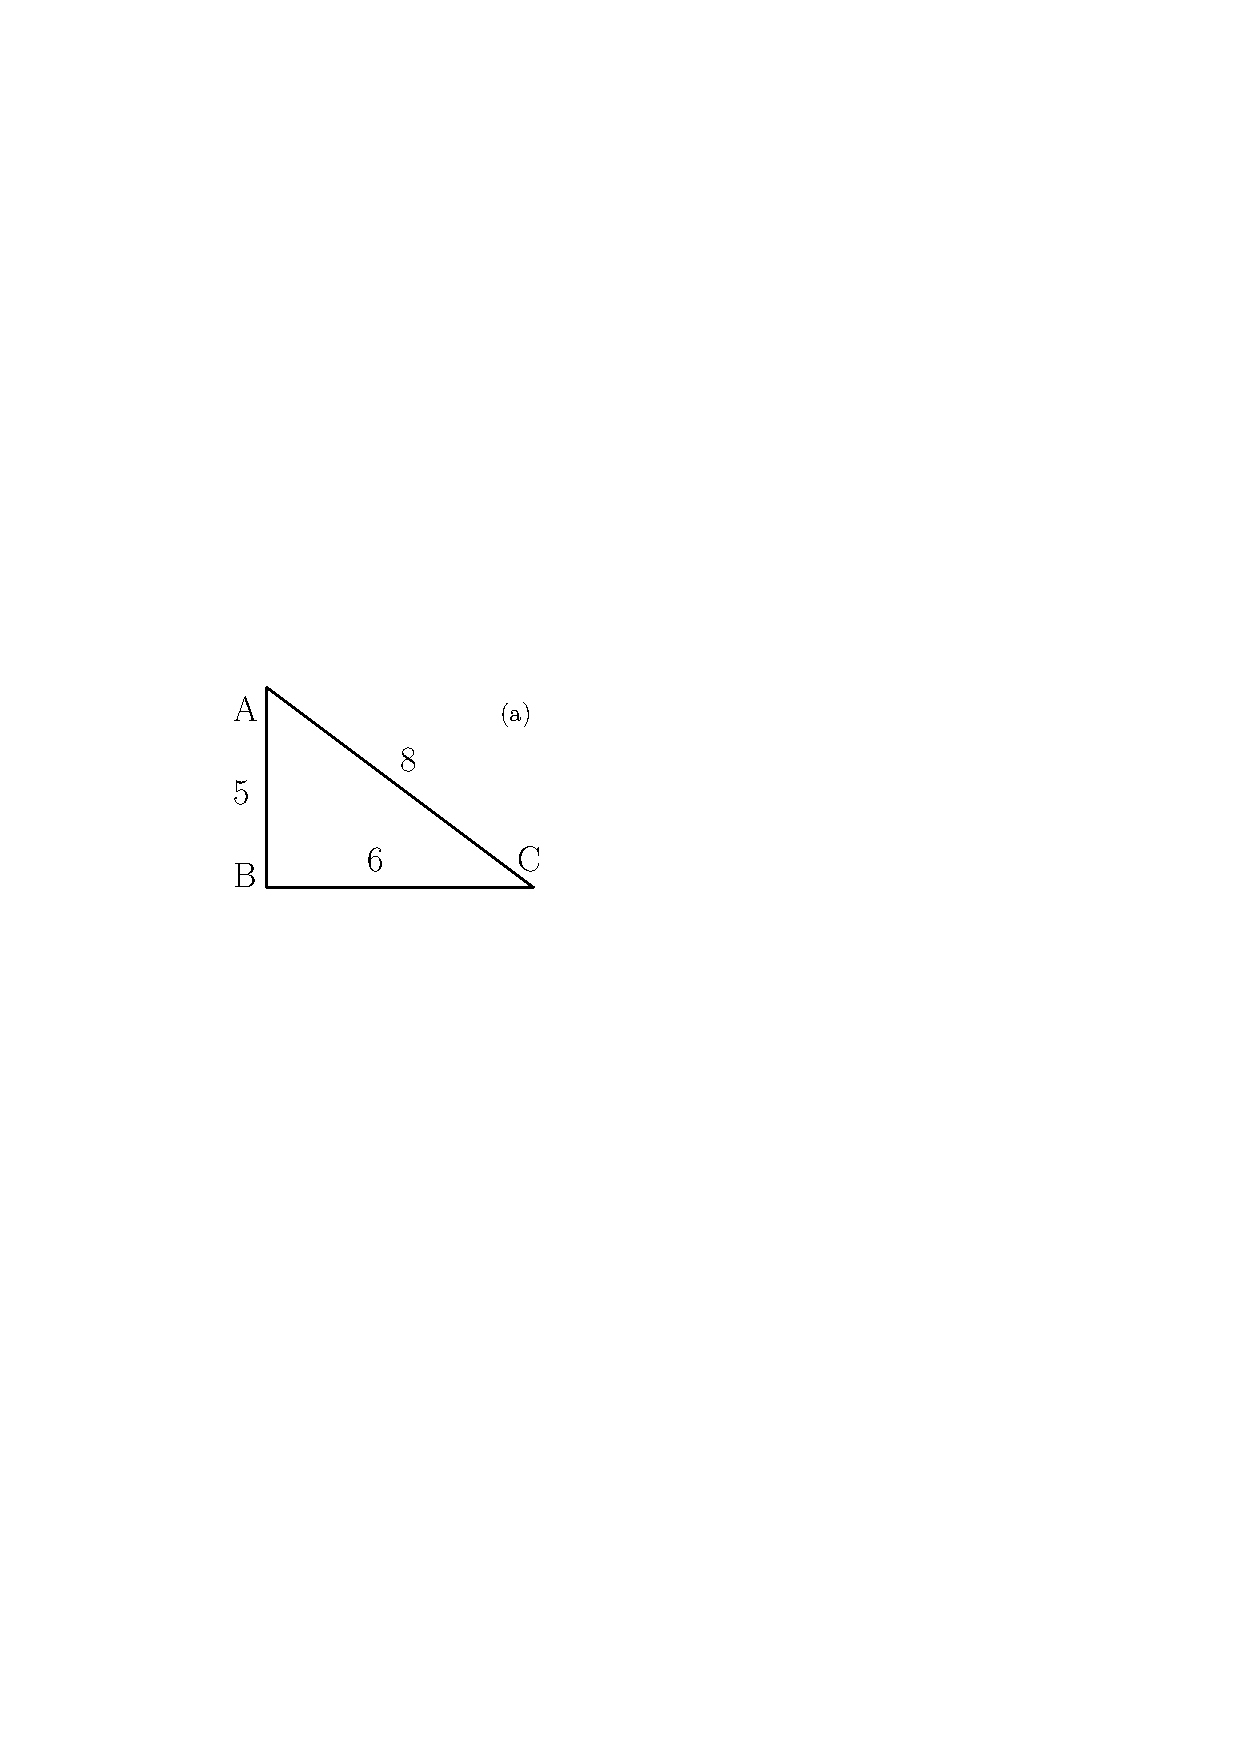
\includegraphics[width=0.7\linewidth]{sources/1/exo2-tri-1a.pdf}
  \end{figure}

  \begin{figure}[H]
    \centering
    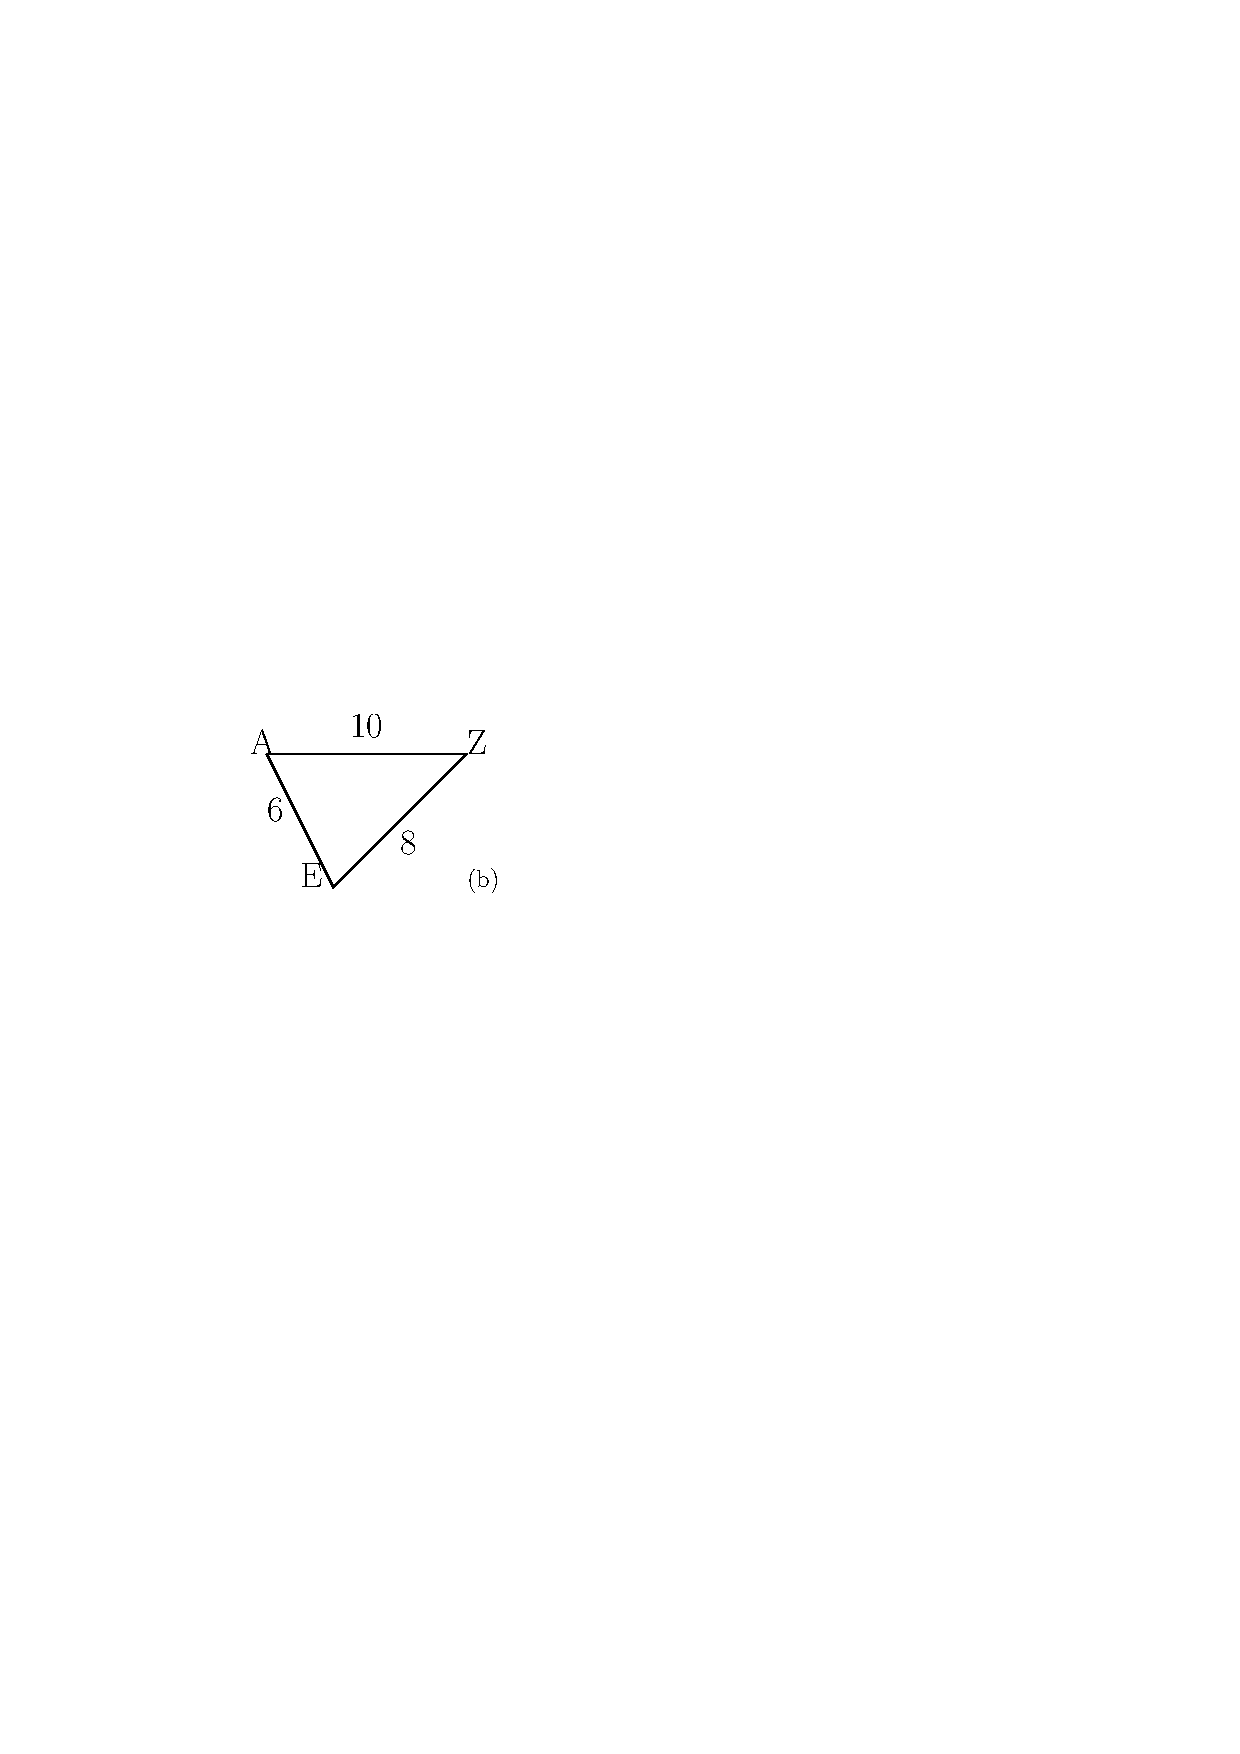
\includegraphics[width=0.7\linewidth]{sources/1/exo2-tri-2.pdf}
  \end{figure}

\end{multicols}

\horrule{1px}

\begin{multicols}{2}

  \subsection*{Exercice 3}
  On sait que le triangle BCD est rectangle en D.\\
  \begin{enumerate}
  \item Calculer BC
  \item Le triangle ABC est-il rectangle ? \textit{Justifier.}
  \end{enumerate}

  \begin{figure}[H]
    \centering
    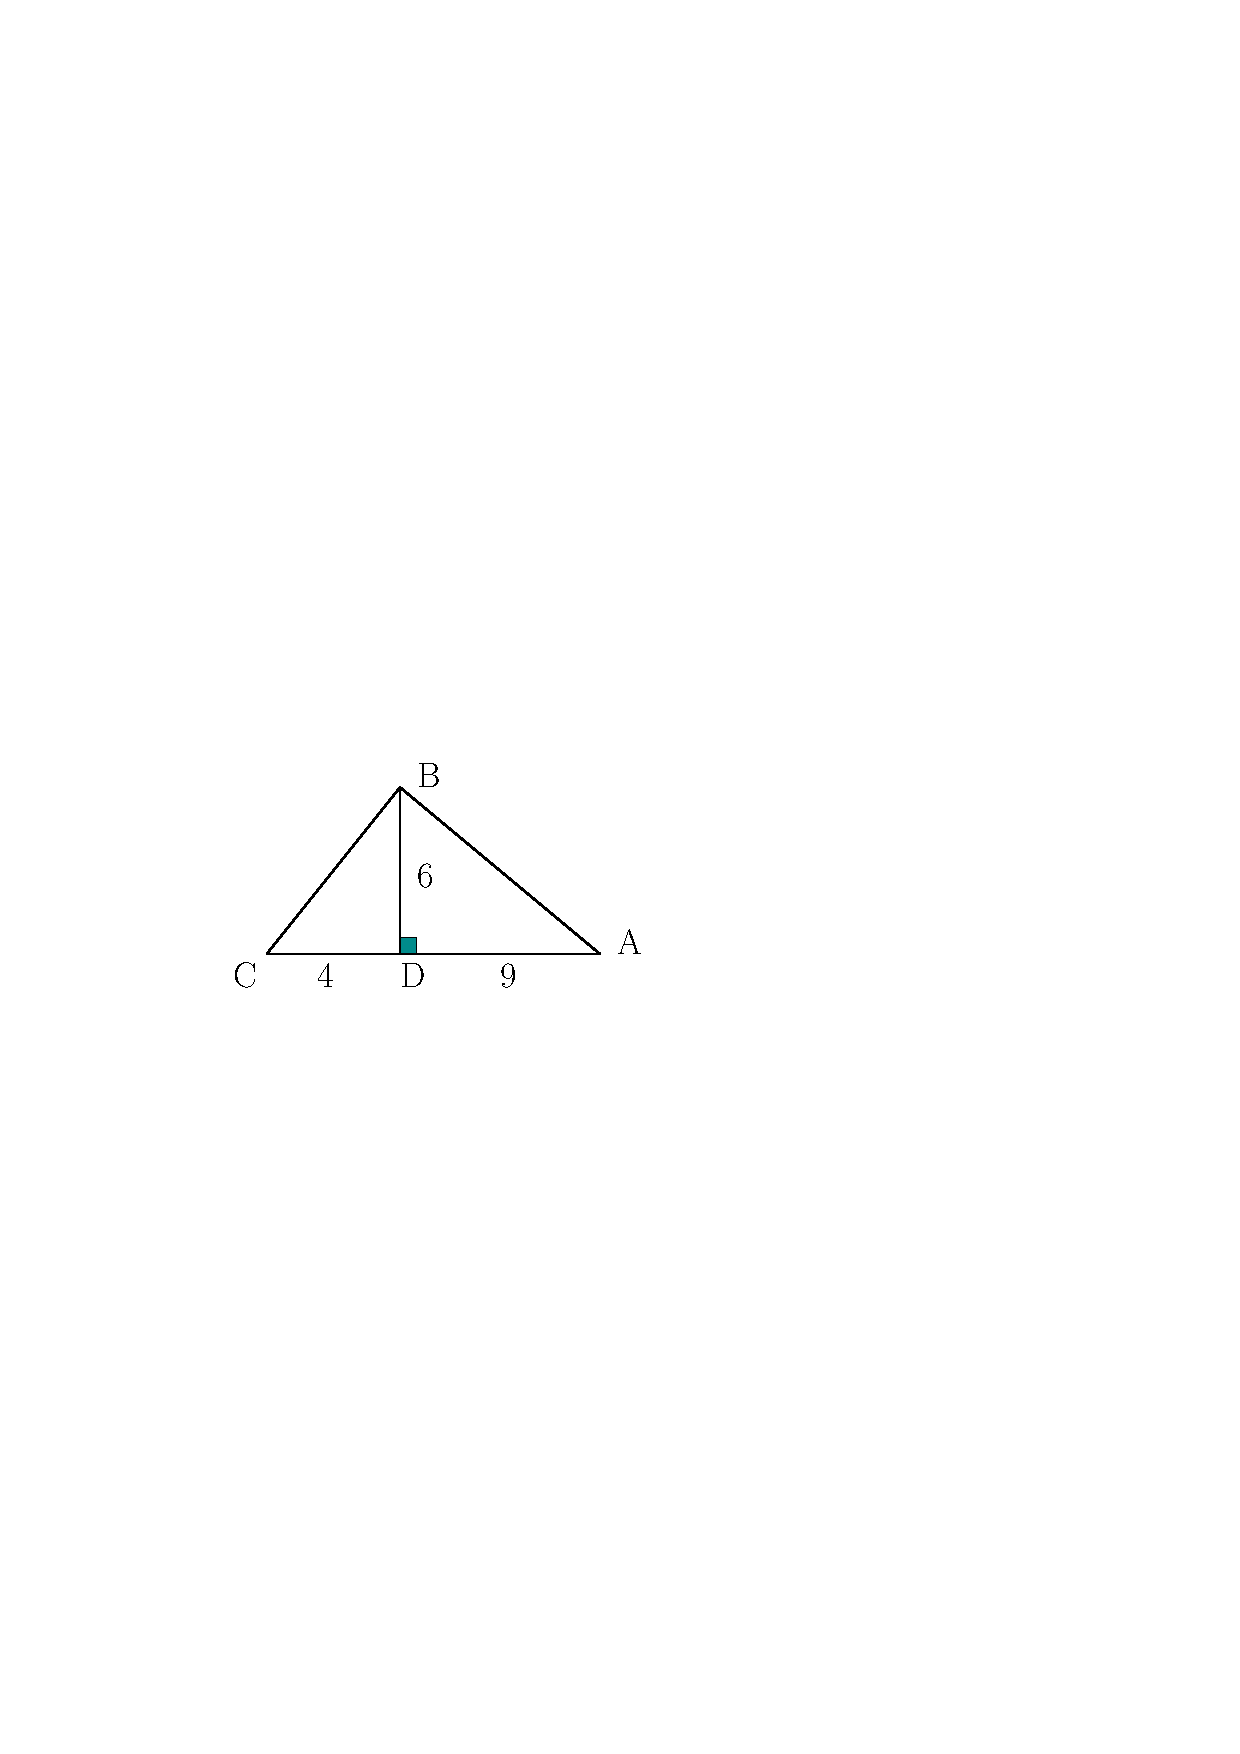
\includegraphics[width=0.7\linewidth]{sources/1/exo3-tria.pdf}
  \end{figure}

\end{multicols}

\horrule{1px}

\begin{multicols}{2}

\subsection*{Exercice 4}

\begin{itemize}
\item Le pont mesure 100m de long. Il est horizontal.
\item Le mat mesure 30m de haut. Il est placé au milieu du pont. Il est vertical. 
\item Des câbles en acier descendent du haut du mat vers le milieu du pont.
\item Des câbles en acier descendent du haut du mat vers l'extrémité du pont.
\end{itemize}

\textbf{Combien de mètre de câble, l'entrepreneur doit-il acheter pour réaliser son pont ?}

\horrule{1px}


\begin{enumerate}
\item[1.] Faire un \textit{beau} schéma avec les longueurs.
\item[2.] Répondre à la question. 
\end{enumerate}
\textit{Remarque : Les câbles en acier sont appelés des haubans.}

\begin{figure}[H]
  \centering
  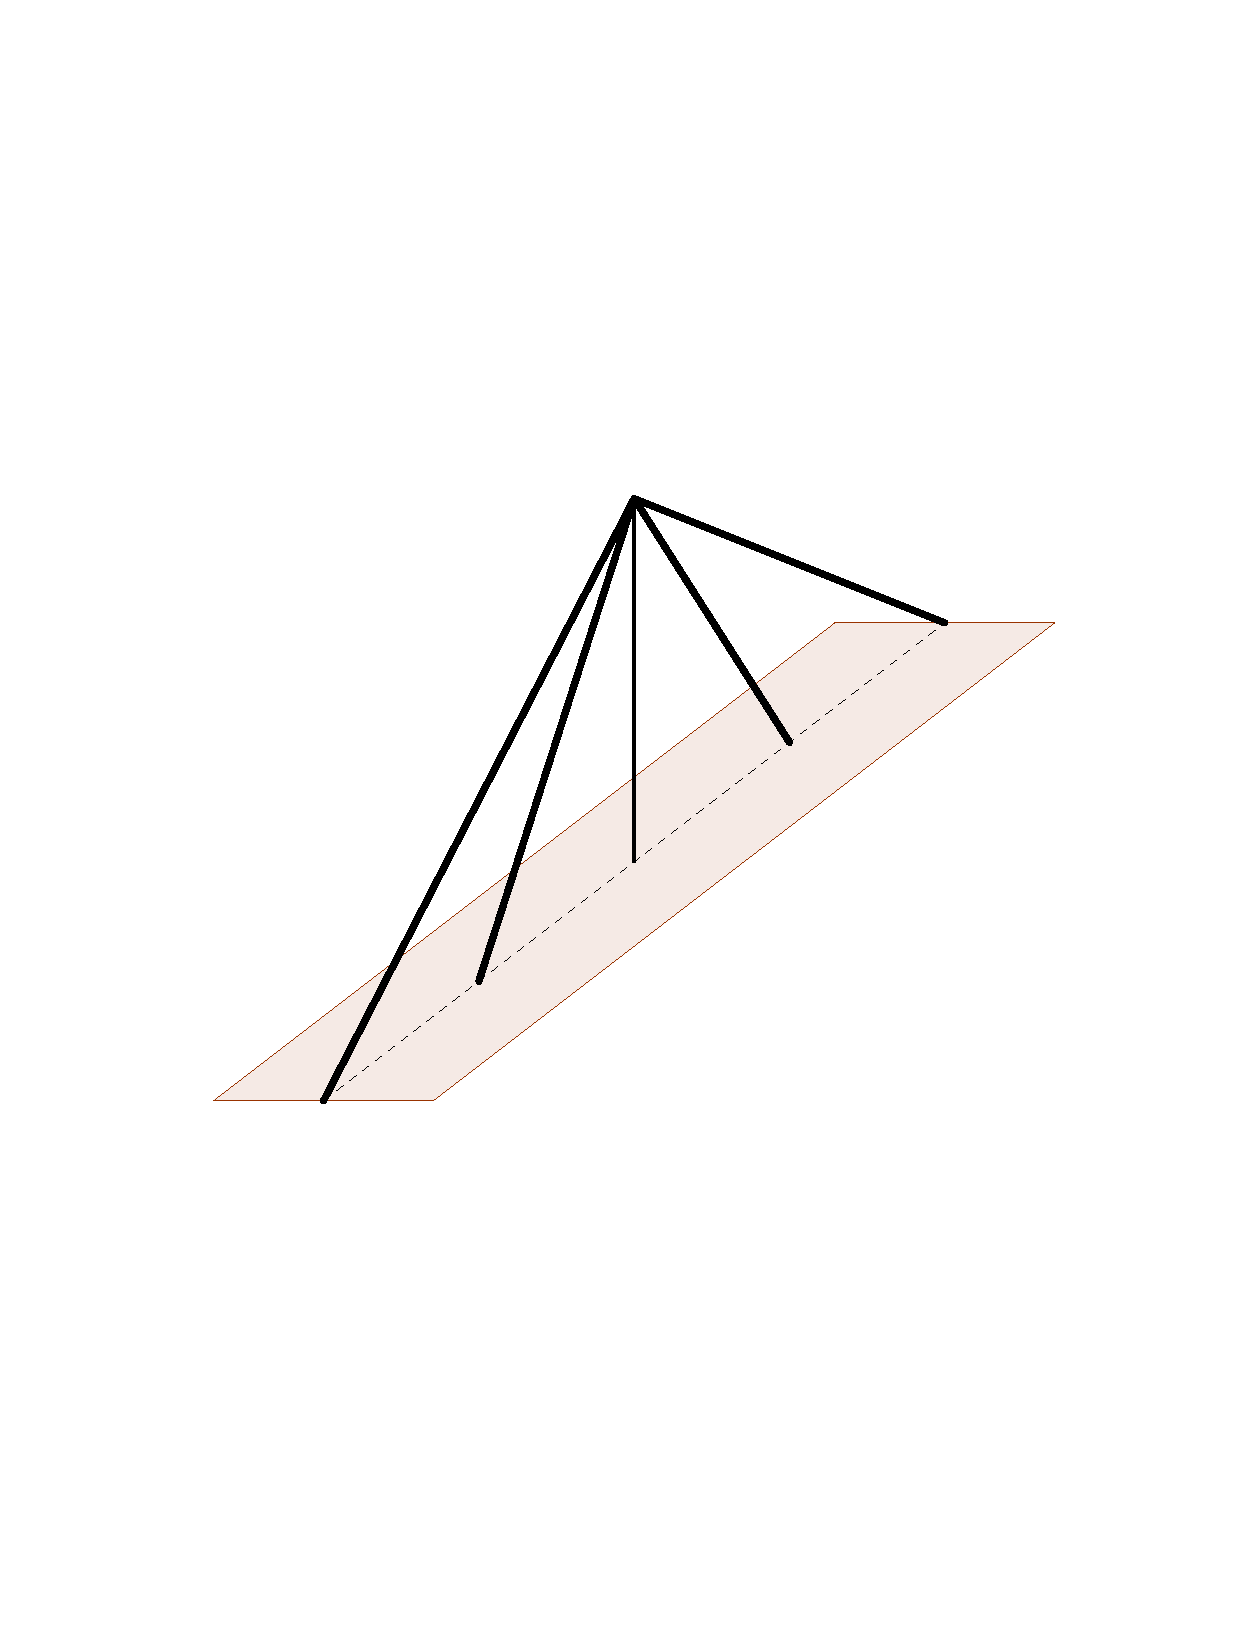
\includegraphics[width=\linewidth, trim={1cm 6cm 1cm 6cm}, clip ]{sources/1/exo-pont-haubans.pdf}
\end{figure}

\end{multicols}

\end{document}
